\chapter{Conceptual Design}
\label{chap:05_design}
%
\todo{Describe Chapter}


% ===========================================
% ===========================================
\section{Design Restrictions}
\label{sec:05_restrictions}
The design of the computing environment will be restricted by several points. These factors are given because of technological choices and requirements from up there.

\begin{itemize}
\item \textbf{Running on a NVIDIA DGX A100\footnote{The Universal System for AI Infrastructure - \url{https://www.nvidia.com/en-us/data-center/dgx-a100/}}:} The environment will run on a NVIDIA DGX A100 workstation. The workstation has 80 CPUs and 8 GPUs installed. For this computing environment, 2 GPUs will be available.

\item Apache Spark: To distribute the workload of training ML models, Apache Spark is a requirement.

\item Python programming language: Python is used as the main programming language for Apache Spark applications. Therefore, examples will use Python code. Configurations for the system are optimized for using Python in production.

\item GitLab: All source code is hosted on a GitLab repository. Additionally, the CI pipeline runs on GitLab CI/CD (introduced in SECTION X).
\end{itemize}

% ===========================================
% ===========================================
\section{Automated Deployment Pipeline}
% Abstract
The objective of this thesis is to automatically submit an Apache Spark application to the Apache Spark cluster to train ML models. Therefore, the training process has to be integrated into the application development lifecycle.
% Git
The source code of an Apache Spark application is hosted on a Git repository. After each committed change on the repository, the pipeline is triggered.


% Conceptual figure
\begin{figure}[h]
\centering
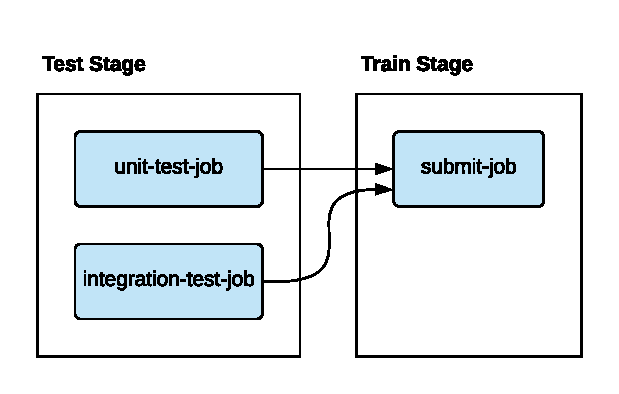
\includegraphics[scale=1]{images/05_conceptual_design/automated_deployment_pipeline/ci_cd_concept}
\caption{Automated Deployment Pipeline concept}
\label{fig:05_deployment_concept}
\end{figure}
% Short intro
\Fig{fig:05_deployment_concept} illustrates the conceptual design of the Automated Deployment Pipeline.
% The stages
The pipeline consists of two different stages:
\begin{enumerate}
\item Test stage: After the build stage has succeeded, the test stage will perform tests.
\item Train stage: If the tests have been successful, the application is submitted to the Apache Spark cluster for training.
\end{enumerate}
% No build stage
It is important to mention, that a build stage is missing in this conceptual design. The build stage includes compiling source code into a format that can be executed directly.
% Python
Python is an interpreted language and therefore no compilation is needed to execute the source code. \todo{Quelle}
% Other languages
As being mentioned in Section SPARK, Apache Spark supports different languages than Python.  For example, for Java application, a build stage is needed to compile the source code to a .jar binary, which can be submitted to the Apache Spark cluster.
% AABBER .egg. zip geht auch bei python
% For Python applications, simply pass a .py file in the place of <application-jar> instead of a JAR, and add Python .zip, .egg or .py files to the search path with --py-files.


\subsection{Test Stage}
% short intro
In order to detect error in an early stage, the source code has to be tested.
% responsibilities
The test stage is responsible to the the source code within a set of various tests. Tests can include:
% Tests
\begin{itemize}
\item Unit tests:
\item Integration tests:
\item End-to-end tests:
\end{itemize}
% Different jobs
For each different test, a new job in the test stage is being created. All jobs will perform in parallel after the test stage has been triggered.
% On failure
If a job has failed, the whole test stage is marked as failure and all participating developers will get a notification.


\subsection{Train Stage}
\paragraph{}
% Short intro
The train stage is responsible to submit the Apache Spark application to the Apache cluster after the test state was successful.
% How
As being mentioned in SECTION XY, an Apache Spark application will be submitted to the Apache Spark cluster by creating a spark-submit Docker container in the same Docker swarm network.
Therefore, after the train stage has been triggered a spark-submit container has to be deployed in the Apache Spark cluster to submit the latest version of the Apache Spark application.

\paragraph{}
% Same machine
To access the Apache Spark cluster Docker swarm network, the train stage has to be executed on the same machine.
% Gitlab runner
Therefore a GitLab runner performing on the machine is needed. Additionally, the GitLab runner needs access to the underlying Docker engine to deploy new container to a given network.
% Perform train stage concept
\begin{figure}[h]
\centering
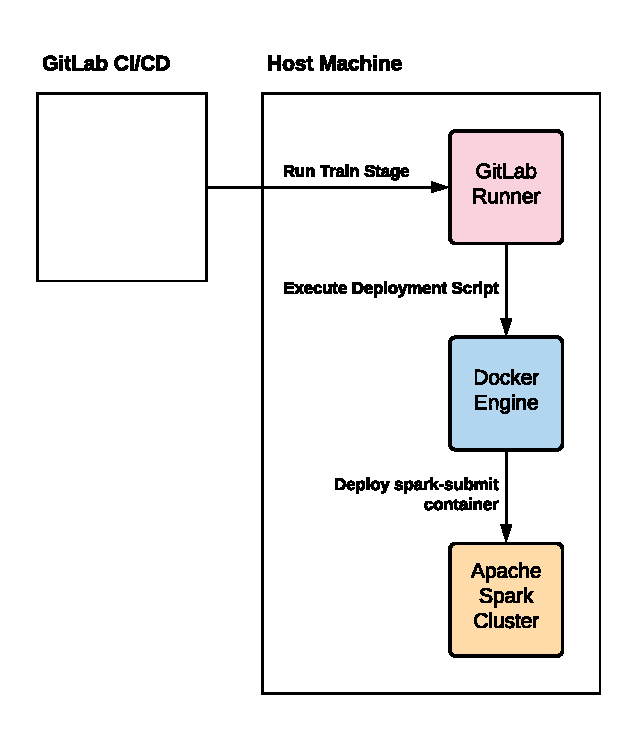
\includegraphics[scale=1]{images/05_conceptual_design/automated_deployment_pipeline/train_stage_runner}
\caption{Deployment of a spark-submit container}
\label{fig:05_deployment_train_concept}
\end{figure}
% Explain figure
\Fig{fig:05_deployment_train_concept} illustrates the steps to deploy a spark-submit container in the Apache Spark cluster swarm network.
% Runner
GitLab CI/CD performs the train stage on the GitLab runner which is running on the NVIDIA DGX machine.
% Deploy
The GitLab Runner executes the deployment script defined in the train stage.
% Deploy script
The deployment script executes a \texttt{docker run} command to deploy a spark-submit container in the Apache Spark cluster swarm network.


% ===========================================
% ===========================================
\section{Identification of Suitable Metrics for Scaling}
% SHort intro
To scale the number of Apache Spark worker in accordance to the actively performing workload, suitable metrics to define the cluster performance have to be defined.
% Rapids enabled GPU
With the RAPIDS accelerator for Apache Spark enabled, the Apache Spark cluster is able to utilize the computing power of GPUs and CPUs to enable parallization.
% SO?
Therefore, suitable metrics to measure the performance are the overall CPU utilization across all worker and the GPU utilization of all available GPUs.
% Those are time-based utilization
These utilization metrics will be based on the time when the Aapche Spark cluster is actively performing computations.


\subsection{CPU Utilization}

%The CPU Utilization means the percentage of time that the CPU runs our program for. Since CPU Utilization is a discrete state, it is not the metric that could reflect on how much power of the CPU we have used, but the proportion of the time our program occupies CPU cycles. That is also why the CPU Utilization can only be raised to 100%, whereas the computational load metric (CPU Load) could go beyond 100%.

%Unlike CPU Utilization, CPU Load could go beyond 100%. The CPU Load metric could give us the actual ‘demand’ of the computer’s resources (not only CPU power), whereas CPU Utilization could only reflect how busy the CPU is. The analogy of the difference between CPU Load and CPU Utilization is the high way traffic. CPU Utilization is how often the freeway is found to have cars running on it, CPU Load is how many cars are demanding the freeway both running on the freeway or waiting to enter the freeway [34]. In Figure 3.2, we can see if the freeway is fully used the CPU Load is 100%, if only half of the freeway is used the CPU Load is 50% and if the freeway is fully used and there are some cars waiting to enter the freeway the CPU Load will go beyond 100% and it is 170% in the figure. In a single core computer like t2.micro, ideally the 100% of the CPU Load indicates that the computational resource is fully utilized and if the value is 200%, it means we need one more instance to handle the load. Since the CPU Load could reflect the overall usage of the resources, the CPU Load could be a crucial performance indicator metric in our fuzzy logic based auto-scaler.

%The CPU Load is initially designed to show the demand of the CPU resource that the task is using the CPU cycles and the task which is waiting to run but not blocked by IO. However the Linux kernel later evolve the CPU Load metric to become different from other non-Linux based operating system. The Linux based operating system will have CPU Load metrics included the TASK UNINTERRUPTIBLE which are the task waiting for IO and locks [35]. Therefore, the CPU Load metric in Linux based operation should be correctly named as the ’System average load’ which represent the demand of the computational resources as whole. Therefore, the CPU Load metric could be a perfect indicator metric for estimating the number of virtual machines needed to satisfy the SLA.

% Sharing CPU cores
All Apache Spark worker run on the same machine. Therefore, all available CPU cores on the machine will be shared across each running Apache Spark worker.


% cadvisor
cAdvisor provides a performance called metric \texttt{container\_cpu\_usage\_seconds\_total}\footnote{Monitoring cAdvisor with Prometheus - \url{https://github.com/google/cadvisor/blob/master/docs/storage/prometheus.md} (Accessed: 2021-01-21)}. This metric provides the total amount of CPU seconds consumed by core per container. 
% Overall utilization
To calculate the overall CPU utilization for all Apache Spark worker, the value of the performance metric for each over a specific rate has to be summed up. Therefore, the CPU utilization ($U_{CPU}$) is defined by:

\begin{equation}
U_{CPU}=\sum_{n=1}^{ActiveWorker}container\_cpu\_usage\_seconds\_total_{n}
\label{eq:formel}
\end{equation}

\subsection{GPU Utilization}
% Number of gpus
Two GPUs on the machine are available across all Apache Spark Worker.
% The metric
The dcgm\_exporter agent provides the \texttt{bla\_bla} performance metric. This metric returns the procentual utilization per GPU.
% How to calculate
Therefore, the overall GPU utilization ($U_{GPU}$) is defined by:


The system has a fixed number of GPUs to use.
\begin{equation}
U_{GPU} = \dfrac{\sum bla\_bla}{ActiveGPUs}
\label{eq:formel}
\end{equation}


% ===========================================
% ===========================================
\section{Computing Environment Architecture}
% Single machine
The computing environment will be deployed on a single machine.
% Autonomic
The goal is to create a self.optimizing environment, according to the autonomic computing environment described in SECTION AB.
% Docker
The be able to scale components in the environment, each components is deployed as a Docker container using Docker Swarm mode (see Section XY). Docker Swarm mode allows to define the number replicas per service an keeps track of it. The number of replicas can be adapted at runtime. This gives the environment an additional self-healing ability.
% Communication
To enable communication, all Docker container run in the same network.

% Overall design
\begin{figure}[h]
\centering
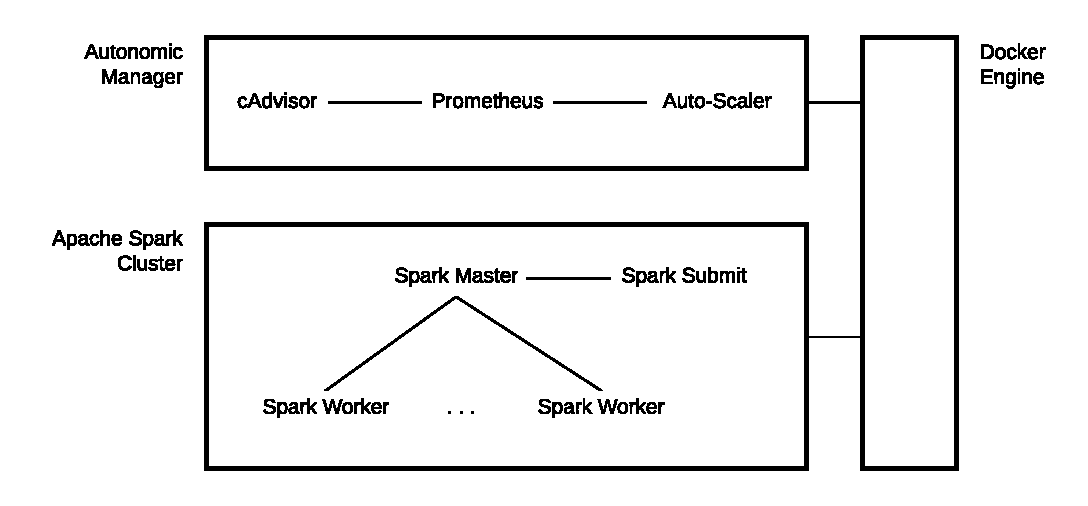
\includegraphics[scale=0.8]{images/05_conceptual_design/cluster_architecture/overall_architecture}
\caption{Overall cluster architecture - Source: Authors own model.}
\label{fig:05_environment_concept}
\end{figure}
% Introduce
\Fig{fig:05_environment_concept} introduces the conceptual architecture of the computing environment.
% Two main components
The computing environment consists of two main modules which consist of individual components:
\begin{itemize}
\item Autonomic manager: Is responsible to automatically monitor the hardware resource utilization of the environment and adapt the number of Apache Spark worker to reach a defined utilization.
\item Apache Spark cluster: An Apache Spark cluster enables to distribute the workload of training ML models. Additionally it enables to perform computation parallel on multiple CPU cores and GPUs.
\end{itemize}
% Managed resources
As being introduced in SECTION XY, an autonomic computing environment consists of an autonomic manager and managed resources.
% Spark are managed resources
In this environment, all Apache Spark worker container are the managed resources.
% Scaling


% ===========================================
% ===========================================
\section{Apache Spark Cluster}
\label{sec:05_spark}
% Short intro
The Apache Spark cluster is the computing unit of the computing environment. It is responsible to distribute the workload of ML training applications.
% Standalone mode
The Apache Spark is deployed in standalone mode. Standalone mode is the most simple mode without the need to install and configure an additional service as a cluster manager. An orchestration tool like Kubernetes or Apache Mesos as cluster manager is not needed, because Docker Swarm mode is used as orchestration tool.
% Docker
Each node in the cluster (Master, Worker, and Submit) will be run as a Docker container.
% Figure
\todo{Figure hier}
% FIgure intro
FIG XY illustrates the Apache Spark cluster architecture. It consists of a single master node, multiple worker nodes, and none or multiple spark-submit nodes.
% worker
The number of worker nodes will be adapted by the Autonomic Manager in accordance to the utilization of defined performance metrics.
% spark-submit
A spark-submit node is only deployed until an application is being submit by the CI pipeline described in SECTION XY.


\subsection{Homogeneous Apache Spark Worker Nodes}
% Short intro
As being mentioned in SECTION AB, horizontal scaling is most efficient by scaling homogeneous node.
% How to achieve
To ensure each worker node is homogeneous, the same Docker image is used for all worker container.
% Resources
This guarantees that each worker has the same resources available and uses the same software as any other worker.


\subsection{Deploying an Application with spark-submit}
% Short intro
A spark-submit node is deployed each time an application is being submitted to the cluster.
% spark-submit purpose
The purpose of a spark-submit node is to submit an application with the spark-submit executable to the cluster (described in SECTION XY).
% No support for python in cluster mode
Standalone mode does not support to submit a Python application with the spark-submit executable from outside of the cluster. Therefore, a node running the spark-submit executable has to be submitted within the cluster \cite{Apache2020Spark}.
% Swarm
To submit and application to the master node, the spark-submit node needs to be in the same Docker swarm network. The node is deployed as a Docker container instead of a Docker service. Each spark-submit node is deployed with a different setting depending on the configuration and application from the CI pipeline.
% End
After the application has been submitted, the spark-submit node automatically exits.

% Was noch evtl fehlt:
% CPU_ONLY mode
% Resourcen für executor einstellen


\subsection{GPU Acceleration with RAPIDS}
One objective of this thesis is, to enable GPU acceleration for Apache Spark.
%
To do this, the RAPIDS accelerator plugin for Apache Spark is being used.
Each worker becomse the same amount of GPU resources.


\section{Autonomic Manager}
\label{05_am}
% SHort intro
The autonomic manager is a main module of the computing environment. The theoretical concept of an autonomic manager is described in SECTION XY.
% Responsibilites
It is responsible to monitor the performance metrics (introduced in SECTION AB) of all Apache Spark worker nodes and automatically scale the number of worker nodes to adapt to a specified performance goal.
% MAPE
The autonomic manager will be implemented according to the MAPE architecture as described in SECTION XY. To create a complete control-loop, the autonomic manager is composed of multiple components as illustrated in \Fig{fig:05_am_concept}.
% A figure explaining the concept
\label{subsec:05_am}
\begin{figure}[h]
\centering
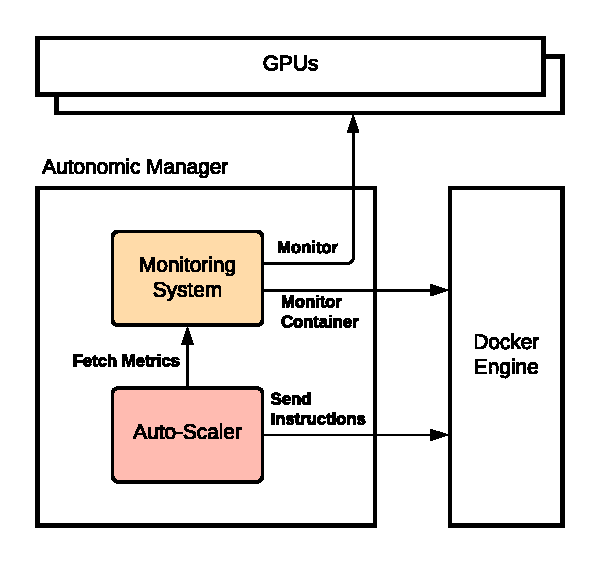
\includegraphics[scale=1]{images/05_conceptual_design/autonomic_manager/autonomic_manager_concept}
\caption{Autonomic manager component design - Source: Authors own model.}
\label{fig:05_am_concept}
\end{figure}
% Explain figure
It consists of a monitoring system (explained in SECTION XY) and an \textit{Auto-Scaler} module.
% Docker
Each component in the computing environment is deployed as a Docker service or container. Therefore, the autonomic manager needs access to the Docker engine to send instructions and monitor performance metrics of Docker container.
% GPU metrics
As being mentioned before, a fixed number of GPUs will be available on the machine. These GPUs need to be monitored on the node level instead of tthe container level. To monitor the GPU utilization, the autonomic manager needs access to the GPUs as well.


\subsection{Monitoring System}
% Short intro
The monitoring system is a main module of the autonomic manager. The tasks of a monitoring system are, to monitor the performance of components in the environment (see SECTION XY).
% Responsibilites
In this environment, the monitoring system collects the performance metrics of the Apache Spark worker Docker container and the GPU performance. It is important to mention that the number of worker nodes varies over time. The Auto-Scaler will scale the replicas of worker nodes according to the system performance.
% Mape
Therefore, it is responsible to perform the Monitor phase of the MAPE architecture.
% CHanging environment
The number of worker node varies over time 
% The figure
\begin{figure}[h]
\centering
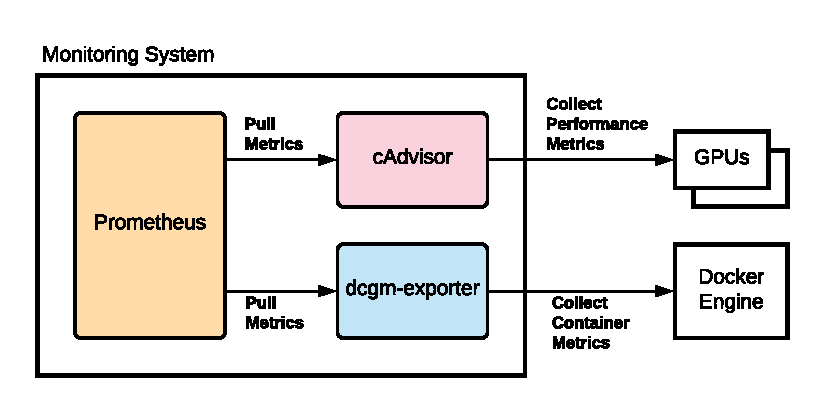
\includegraphics[scale=1]{images/05_conceptual_design/autonomic_manager/monitoring_system_concept}
\caption{Autonomic manager component design - Source: Authors own model.}
\label{fig:05_am_monitoring_concept}
\end{figure}
% Explain figure
\Fig{fig:05_am_monitoring_concept} illustrates the architecture of the monitoring system. It consists of three components:
% The components
\begin{itemize}
\item dcgm-exporter: A monitoring agent which is responsible to collect GPU performance metrics.
\item cAdvisor: cAdvisor is monitoring agent which collects performance metrics of Docker container in the environment.
\item Prometheus: Prometheus collects the performance metrics from all monitoring agents and saves them as time-series data in a time-series database.
\end{itemize}
% Docker
Each component will be deployed as a Docker service in the overall Docker swarm.


\subsection{Auto-Scaler}
% Short intro
The \textit{Auto-Scaler} is the second module of the autonomic manager and responsible to dynamically adjust the replicas of Apache Spark worker nodes in the computing environment to accommodate specified performance goals.
% MAPE
It implements the Analyse, Plan, and Execute phases of the MAPE architecture.
% MAPE
In addition to the monitoring system, the Auto-Scaler creates a complete autonomic manager implementing all four phases of the MAPE architecture.
% Reactive threshold based 
The \textit{Auto-Scaler} is a reactive auto-scaler (described in SECTION XY) and used a threshold-based algorithm to adapt the number of worker nodes.
% Prom API
As illustrated in \Fig{fig:05_am_concept}, the \textit{Auto-Scaler} fetches performance metrics from the monitoring system.
% Prom API
To fetch metrics from the monitoring-system, it connects to the HTTP API of Prometheus.
% Phases
After it received the performance metrics, the Auto-Scaler analyses the metrics, plans scaling-actions to adjust the number of worker replicas and sends instructions to the Docker engine.
% Configuration
The \textit{Auto-Scaler} can be configured using a configuration file.


\subsubsection{MAPE Phases}
% SHort intro
As being mentioned, the \textit{Auto-Scaler} implements the Analyse, Plan, and Execute phases of the MAPE architecture. Each phase has a different workflow to accommodate its goal.

\paragraph{Analyse:}
% Short intro to analyze phase
In order to determine if a scaling-action is necessary, the \textit{Auto-Scaler} has fetch and analyse all defined performance metrics. 
% How to analyze
During each period, the \textit{Auto-scaler} fetches performance metrics from the Prometheus HTTP API with specified PromQL queries.
% Determine if scaling is needed
After the metrics are received, the \textit{Auto-Scaler} determines if a scaling action is needed using the Scaling Heat algorithm (introduced in Section AB). If scaling is not necessary, the \textit{Auto-Scaler} continues to collect and analyse performance metrics from Prometheus.

\paragraph{Plan:}
% Short intro
If a scaling-action is necessary, the \textit{Auto-Scaler} is responsible to determine the number of Apache Spark worker replicas, needed to reach the utilization goals.
% What is a scaling plan
A scaling plan consists of instructions to add or remove worker nodes. These instructions are send to the Docker engine.
% Calculating Spark worker
To calculate the number of worker nodes, the \textit{Auto-Scaler} uses the Kubernetes Horizontal Pod Auto-Scaling algorithm (introduced in SECTION XY).
% Thresholds
In addition, the Auto-Scaler needs to check if the estimated number of worker replicas violate the specified upper- and lower-thresholds of active worker nodes.

\paragraph{Execute:}
% Short intro
After a scaling plan is created, the Auto-Scaler needs to send the instructions to the Docker engine.
% Cooldown
After scaling the number of worker replicas, the Apache Spark cluster needs time for changes to take effect. Therefore, a cooldown period is activated after each scaling action (explained in Section AB).
% Whats happens
During the cooldown period, no scaling actions are executed.


\subsubsection{Configuration}
\label{subsubsec:05_am_auto-scaler_config}
The Auto-Scaler needs specific configuration properties to be able to collect the correct metrics from Prometheus and deploy new Apache Spark worker container in the environment. The following are properties that have to be defined to ensure that the Auto-Scaler is able to collect meaningful metrics and scale Apache Spark worker as expected.

\begin{itemize}
\item General properties:
\begin{itemize}
\item Interval seconds: The number of seconds when the loop has to repeat needs to be defined.

\item Cooldown period: The duration in seconds,  the Auto-Scaler has to wait after a scaling action was performed.

\item Recurrence factor: To prevent to many scaling actions,  the autonomic manager should only execute a scaling action,  if the utilization thresholds is violated \textit{n} times.

\item Prometheus URL: The Auto-Scaler will fetch the configured metrics from the Prometheus REST API.
\end{itemize}

\item Metrics:
To support to analyze multiple metrics, the user should be able to create a dynamic list if metrics. Each metric needs to have a variety of properties configured.
\begin{itemize}
\item Target utilization: The relative target utilization of a metrics needs to be defined to calculate the number of Spark worker to add or to remove to reach the defined goal.

\item Utilization thresholds: To determine if a scaling action is needed, the scaling heat algorithm needs the minimum and maximum utilization defined by an administrator.

\item Query: A PromQL query needs to be defined to collect the metric for all Spark Worker.
\end{itemize}

\item Apache Spark worker properties:
\begin{itemize}
\item Worker image: To guarantee that each Spark worker is homogeneous, all worker container should be created with the same image.

\item Worker network: To establish communication between all Spark worker and the Spark master, all new Spark worker container should be in the same network.

\item Worker thresholds: The minimum and maximum number of concurrent Spark worker should be defined. To avoid the cold start effect, the minimum amount of worker should be 1. 

\item Apache Spark master URI: To distribute the workload across all Spark Worker, all Spark Worker need to communicate with the Spark master.
\end{itemize}
\end{itemize}


\subsection{Control Loop}
\paragraph{}
% The control loop
\begin{figure}[h]
\centering
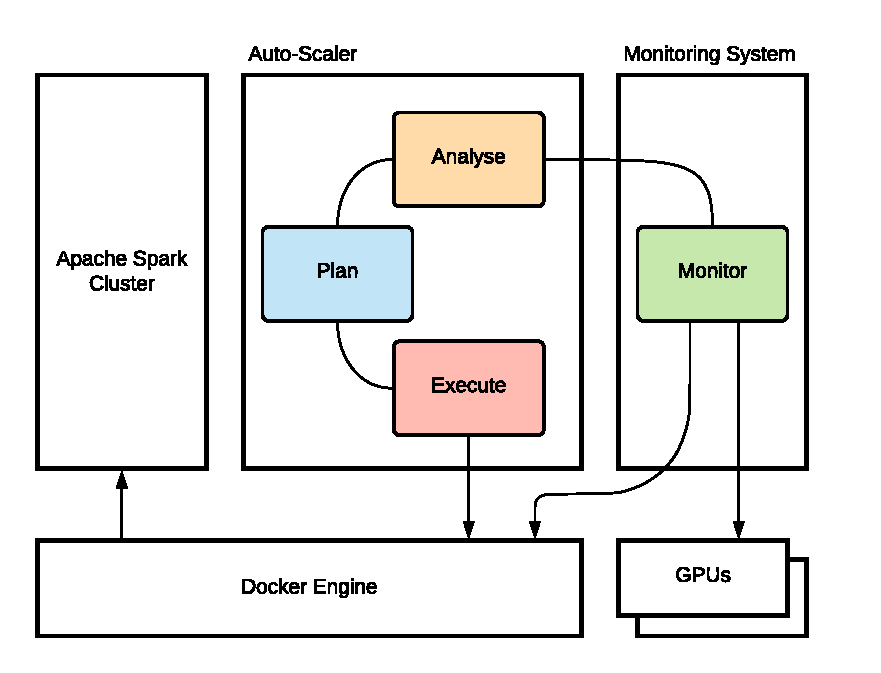
\includegraphics[scale=1]{images/05_conceptual_design/autonomic_manager/control_loop}
\caption{Full MAPE control loop architecture}
\label{fig:05_am_monitoring_loop_arch}
\end{figure}
% Explain 
\Fig{fig:05_am_monitoring_loop_arch} provides an overview about the complete control loop
% Each phases
The monitoring system monitors performance metrics from Docker containers and the GPUs on the machine.
% Auto-scaler
Next, the Auto-Scaler analyses the performance metrics, creates scaling plans and sends instructions to the Docker engine to scale the Apache Spark cluster.


\paragraph{}
% Workflow figure
\begin{figure}[h]
\centering
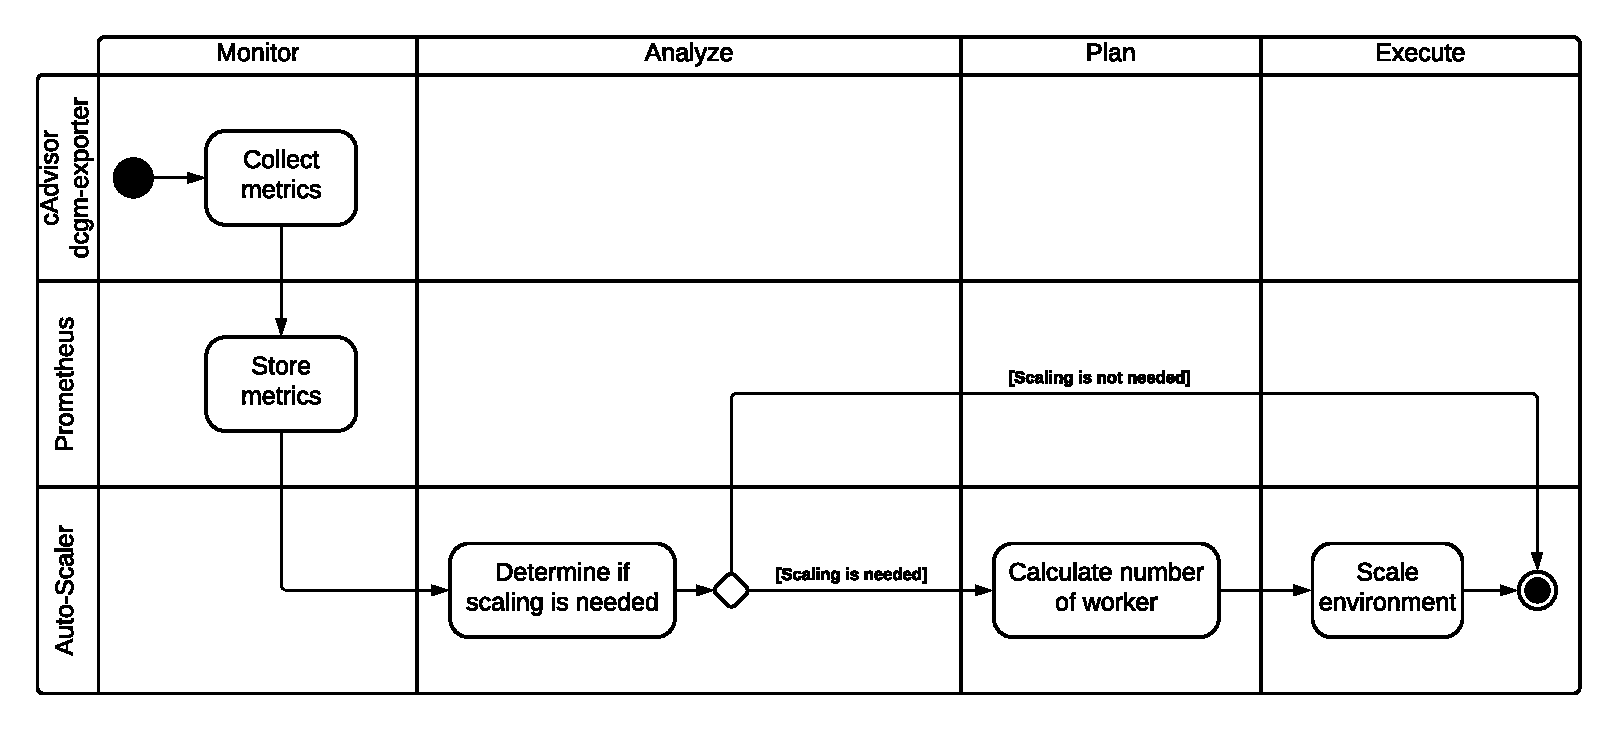
\includegraphics[scale=0.50]{images/05_conceptual_design/autonomic_manager/autonomic_manager_workflow}
\caption{UML activity model of the autonomic manager process - Source: Authors own model.}
\label{fig:05_am_monitoring_loop_workflow}
\end{figure}
% Explain
The control-loop workflow is illustrated in \Fig{fig:05_am_monitoring_loop_workflow}.
% Monitor
It starts in the Monitor phase. All monitoring agents (cAdvisor and dcgm-exporter) collect performance metrics from their targets. Next, Prometheus pulls the metrics from all monitoring agents and saves the data in its time-series database.
% Analyze
In the analyse phase, the Auto-scaler determines if a scaling action is necessary. If a scaling action is not needed, the workflow ends and starts again in the Monitor phase in the iteration.
% Plan
Otherwise if a scaling action is needed, the Auto-Scaler determines the number of Apache Spark worker replicas in the Plan phase.
% Execute
Lastly, in the Execute phase, the Auto-scaler scales the Apache Spark worker nodes.
